\clearpage

\chapter{\documentName}
\section{\documentName}

\testimonial

The original assignment can be found \pdflink{\AssDir Assignment 1B - Informed Search.pdf}{here}.

% Problem
\begin{problem}{Problem 1}
    \begin{statement}{Problem Statement}
        Consider the state space graph shown below. A is the start state and G is the goal state. The costs for each edge are shown on the graph. Each edge can be traversed in both directions. Note that the heuristic $h_{1}$ is consistent but the heuristic $h_{2}$ is not consistent.

        \begin{center}
            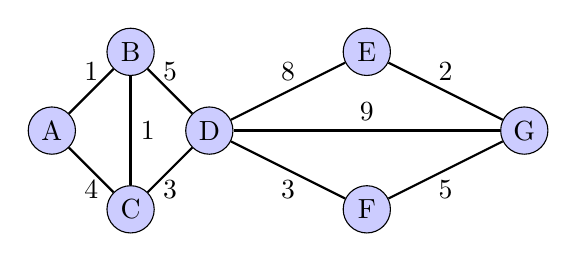
\begin{tikzpicture}
                [node/.style={circle, draw, fill=blue!20, minimum size=6mm, inner sep=0pt}, edge/.style={draw, thick}]
                % Define nodes
                \node[node] (A) at (0,0) {A};
                \node[node] (B) at (1,1) {B};
                \node[node] (C) at (1,-1) {C};
                \node[node] (D) at (2,0) {D};
                \node[node] (E) at (4,1) {E};
                \node[node] (F) at (4,-1) {F};
                \node[node] (G) at (6,0) {G};
                % Define edges
                \draw[edge] (A) -- (B) node[midway, above] {1};
                \draw[edge] (A) -- (C) node[midway, below] {4};
                \draw[edge] (B) -- (C) node[midway, right] {1};
                \draw[edge] (B) -- (D) node[midway, above] {5};
                \draw[edge] (C) -- (D) node[midway, below] {3};
                \draw[edge] (D) -- (E) node[midway, above] {8};
                \draw[edge] (D) -- (F) node[midway, below] {3};
                \draw[edge] (D) -- (G) node[midway, above] {9};
                \draw[edge] (E) -- (G) node[midway, above] {2};
                \draw[edge] (F) -- (G) node[midway, below] {5};
            \end{tikzpicture}
            \hspace{10pt}
            \begin{tabular}[b]{|c|c|c|}
                \hline Node & $h_{1}$ & $h_{2}$ \\ \hline
                A & 9.5 & 10 \\
                B & 9 & 12 \\
                C & 8 & 10 \\
                D & 7 & 8 \\
                E & 1.5 & 1 \\
                F & 4 & 4.5 \\
                G & 0 & 0 \\ \hline
            \end{tabular}
        \end{center}
        \begin{enumerate}[label = {\textbf{(\alph*)}}]
            \item \textbf{Possible Paths Returned}
            
            For each of the following graph search strategies (\textit{do not answer for tree search}), mark which, if any, of the listed paths it could return. Note that for some search strategies 
            the specific path returned might depend on tie-breaking behavior. In any such cases, make sure to mark \textit{all} paths that could be returned under some tie-breaking scheme.

            \begin{center}
                \begin{tabular}[h]{|c|c|c|c|}
                    \hline Search Algorithm & \textbf{A-B-D-G} & \textbf{A-C-D-G} & \textbf{A-B-C-D-F-G} \\ \hline
                    Depth First Search & & & \\ \hline
                    Breadth First Search & & & \\ \hline
                    Uniform Cost Search & & & \\ \hline
                    A$^{*}$ Search With Heuristic $h_{1}$ & & & \\ \hline
                    A$^{*}$ Search With Heuristic $h_{2}$ & & & \\ \hline
                \end{tabular}
            \end{center}
            \item \textbf{Heuristic Function Properties}
            
            Suppose you are completing the new heuristic function $h_{3}$ shown below. All the values are fixed except $h_{3}(B)$.

            \begin{center}
                \begin{tabular}[h]{|c|c|c|c|c|c|c|c|}
                    \hline Node & A & B & C & D & E & F & G \\ \hline
                    $h_{3}$ & 10 & ? & 9 & 7 & 1.5 & 4.5 & 0 \\ \hline
                \end{tabular}
            \end{center}
            For each of the following conditions, write the set of values that are possible for $h_{3}(B)$. For example, to denote all non-negative numbers, write $[0, \infty]$, to denote the empty set, write $\varnothing$, and so on.

            \begin{enumerate}[label = {\textbf{(\roman*)}}]
                \item \textbf{What values of $h_{3}(B)$ make $h_{3}$ admissible?}
                \item \textbf{What values of $h_{3}(B)$ make $h_{3}$ consistent?}
                \item \textbf{What values of $h_{3}(B)$ will cause A$^{*}$ graph search to expand node A, then node C, then node B, then node D in order?}
            \end{enumerate}
        \end{enumerate}
    \end{statement}

    \clearpage

    \begin{highlight}[Part A - Solution]
        \subsubsection*{Depth First Search}

        All of the paths that are listed in this table are able to be explored using Depth First Search. This is because the graph that we are working with does not have any directions. Because this graph is undirected,
        the paths that are listed in the table are absolutely possible. For Depth First Search we can then say: \vspace*{1em}

        \begin{center}
            \begin{tabular}[h]{|c|c|c|c|}
                \hline Search Algorithm & \textbf{A-B-D-G} & \textbf{A-C-D-G} & \textbf{A-B-C-D-F-G} \\ \hline
                Depth First Search & Yes & Yes & Yes \\ \hline
            \end{tabular}
        \end{center}

        \subsubsection*{Breadth First Search}
        
        The only path for Breadth First Search that is not possible to be traversed is \textbf{A-B-C-D-F-G}. This is because of the nature of Breadth First Search. Starting from A, BFS will then visit 
        all children of A first. After the children are visited, the next level of children are visited after that. In the path \textbf{A-B-C-D-F-G}, if we first visited B, we would essentially be revisiting
        C for this path to be valid. And this is not a valid search done by BFS since we cannot revisit children. For Breadth First Search we can then say:

        \begin{center}
            \begin{tabular}[h]{|c|c|c|c|}
                \hline Search Algorithm & \textbf{A-B-D-G} & \textbf{A-C-D-G} & \textbf{A-B-C-D-F-G} \\ \hline
                Breadth First Search & Yes & Yes & No \\ \hline
            \end{tabular}
        \end{center}

        \subsubsection*{Uniform Cost Search}

        Uniform Cost Search is always going to return the path that has the least cumulative cost out of all possible paths. The first path, \textbf{A-B-D-G} is going to have a cumulative cost of 15, 
        \textbf{A-C-D-G} is going to have a cumulative cost of 16, and the final path is going to have a cumulative cost of \textbf{A-B-C-D-F-G} will have a cumulative cost of 13. This means the only path
        that can be returned using UCS is going to be \textbf{A-B-C-D-F-G}. For Uniform Cost Search we can then say:

        \begin{center}
            \begin{tabular}[h]{|c|c|c|c|}
                \hline Search Algorithm & \textbf{A-B-D-G} & \textbf{A-C-D-G} & \textbf{A-B-C-D-F-G} \\ \hline
                Uniform Cost Search & No & No & Yes \\ \hline
            \end{tabular}            
        \end{center}

        \subsubsection*{A$^{*}$ Search With Heuristic $h_{1}$}

        For each heuristic, both $h_{1}$ and $h_{2}$, we essentially need to calculate 

        \begin{center}
            \begin{highlightbox}
                f(\alpha) = g(\alpha) + h(\alpha)
            \end{highlightbox}
        \end{center}
        where $\alpha$ is a node in the graph. Conversely, $g(\alpha)$ is the cost to arrive at a specific node. A$^{*}$ Search is going to prioritize the path that has the lowest $f$ cost. Keeping this in mind,
        the path that has the lowest $f$ cost of all three paths is \textbf{A-B-C-D-F-G} with $f(G) = 13$. Conversely \textbf{A-B-D-G} is $f(G) = 15$ and \textbf{A-C-D-G} is $f(G) = 16$. For A$^{*}$ Search with 
        heuristic $h_{1}$ we can say:

        \begin{center}
            \begin{tabular}[h]{|c|c|c|c|}
                \hline Search Algorithm & \textbf{A-B-D-G} & \textbf{A-C-D-G} & \textbf{A-B-C-D-F-G} \\ \hline
                A$^{*}$ Search With Heuristic $h_{1}$ & No & No & Yes \\ \hline
            \end{tabular}   
        \end{center}

        \subsubsection*{A$^{*}$ Search With Heuristic $h_{2}$}

        Similar to heuristic $h_{1}$, we need to find the path with the smallest $f$ value. For the path \textbf{A-B-D-G} we have $f(G) = 15$, \textbf{A-C-D-G} is $f(G) = 16$, and lastly \textbf{A-B-C-D-F-G}
        has an $f$ value of $f(G) = 13$. A$^{*}$ will once again choose the path with the smallest $f$ value.

        \begin{center}
            \begin{tabular}[h]{|c|c|c|c|}
                \hline Search Algorithm & \textbf{A-B-D-G} & \textbf{A-C-D-G} & \textbf{A-B-C-D-F-G} \\ \hline
                A$^{*}$ Search With Heuristic $h_{2}$ & No & No & Yes \\ \hline
            \end{tabular}   
        \end{center}
    \end{highlight}

    \clearpage

    \begin{highlight}[Part B - Solution]
        \begin{enumerate}[label = {\textbf{(\roman*)}}]
            \item To determine what values of $h_{3}(B)$ make $h_{3}$ \textit{admissible}, we need to not overestimate the cost using
            
            \begin{center}
                \begin{highlightbox}
                    f(\alpha) = g(\alpha) + h(\alpha)
                \end{highlightbox}
            \end{center}
            where $g(\alpha)$ is the cost to get to a current node and $h(\alpha)$ is the estimated cost to get from the current node to the goal. We essentially need to find the most minimal cost for
            going from B to G out of all possible paths. The possible costs from B to G are: 

            \begin{itemize}
                \item \textbf{B-D-G}: Cost is 14
                \item \textbf{B-D-E-G}: Cost is 15
                \item \textbf{B-D-F-G}: Cost is 13
                \item \textbf{B-C-D-G}: Cost is 13
                \item \textbf{B-C-D-E-G}: Cost is 14
                \item \textbf{B-C-D-F-G}: Cost is 12
            \end{itemize}
            Therefore, we must take the minimum of these possible costs. This means the \textit{admissible} values for $h_{3}(B)$ are

            \begin{center}
                \begin{highlightbox}
                    h_{3}(B) = (0,12].
                \end{highlightbox}
            \end{center}

            \item To determine what values of $h_{3}(B)$ make $h_{3}(B)$ \textit{consistent}, we need to take the minimal cost in terms of heuristic values for expanding from node B. The value that we
            are essentially calculating is

            \begin{center}
                \begin{highlightbox}
                    h_{3}(n_{1}) - h_{3}(n_{2}) \leq g(n_{1}, n_{2})
                \end{highlightbox}
            \end{center}
            The neighbors of B are A,C, and D. Going through these calculations for each B's neighbors we find

            \begin{itemize}
                \item $h_{3}(B) \leq g(B,A) + h_{3}(A) \leq 1 + 10 \leq 11 \hspace*{20pt} h_{3}(B) \geq h_{3}(A) - g(A,B) \geq 10 - 1 \geq 9$
                \item $h_{3}(B) \leq g(B,C) + h_{3}(C) \leq 1 + 9 \leq 10 \hspace*{20pt} h_{3}(B) \geq h_{3}(C) - g(C,B) \geq 9 - 1 \geq 8$
                \item $h_{3}(B) \leq g(B,D) + h_{3}(D) \leq 5 + 7 \leq 12 \hspace*{20pt} h_{3}(B) \geq h_{3}(D) - g(D,B) \geq 7 - 5 \geq 2$
            \end{itemize}
            This means for $h_{3}$ to be \textit{consistent}, we must restrict its values to be

            \begin{center}
                \begin{highlightbox}
                    h_{3}(B) = [9,10].
                \end{highlightbox}
            \end{center}

            \item To determine the value of $h_{3}(B)$ that will generate the path \textbf{A-C-B-D} \dots we first have to ensure that we expand C first from A. This is only possible if the corresponding
            $f$ value that is produced when expanding to C is less than that of B. At this point in time, if we first expand to C then

            \begin{equation*}
                f(C) = g(A,C) + h_{3}(C) = 4 + 9 = 13.
            \end{equation*}
            This in turn means that 

            \begin{equation*}
                f(B) > f(C) > g(A,B) + h_{3}(B) > 1 + h_{3}(B) > 13 \hspace*{10pt} \rightarrow \hspace*{10pt} h_{3}(B) > 12.
            \end{equation*}
            To now travel from C to B we constitute $f(B) < f(D)$. At this point in time we then have in our path

            \begin{equation*}
                f(D) = g(C,D) + h_{3}(D) = 7 + 7 = 14.
            \end{equation*}
            So, now applying $f(B) < f(D)$ this means

            \begin{equation*}
                f(B) < f(D) < g(C,B) + h_{3}(B) < 5 + h_{3}(B) < 14 \hspace*{10pt} \rightarrow \hspace*{10pt} h_{3}(B) < 9.
            \end{equation*}
            At this point we have a contradiction; $h_{3}(B)$ must be greater than 12 and less than 9 for this path to happen. \textbf{This is not possible}.
        \end{enumerate}
    \end{highlight}
\end{problem}